% TODO: Get a citation for better attentivity => better information recall.
\section{User Study}
	\subsection{Overview}
	A study was performed in which the change in user engagement was measured upon being presented with interactive and non-interactive advertisements. To estimate user engagement, we measured the participants time perception, known to indicate engagement \citep{yahoo-intrusive-advertising}, and information recall, known to correlate with attention \citep{interactions_attention_memory}--an indicator of engagement \cite{what_is_engagement}.

	\subsection{Methodology}
	Using a set of 119 student targeted adverts taken from Project4, 8 were given interactive html/css overlays containing interactive content likely to be typical for an interactive TV advert. Each participant in the study was shown two rounds of adverts---one interactive and one non-interactive---with half the participants being shown the interactive adverts first, and the other half shown non-interactive adverts first. The length of the rounds varied between 4, 5, and 6 minutes, and were evenly split between longer interactive rounds, longer non-interactive rounds and equal length rounds; the purpose of which was to measure differences in the participants perceived time and actual round time. 

	The study was scripted, which has been included in Appendix~\ref{sec:appendix_interview_script}. While participants were neither encouraged nor discouraged from interacting with the interactive set of adverts, they were informed that interactions were possible, and how to interact, removing the initial learning period. As part of the study, an video introduction was given, which is included in Appendix~\ref{sec:appendix_video_script}.
	\begin{table}[hb]
		\centering
		\begin{tabularx}{\linewidth}{ c X }
			\toprule
			\bf Product & \bf Interactive content \\
			\midrule
			Pot Noodle & \textbf{Poll}: The user is encouraged to vote for their favourite flavour of pot noodle. \\
			Smirnoff Vodka & \textbf{Social}: The user may `like' the product, interacting with the social networking website Facebook. \\ % TODO: do.
			Movie & \textbf{Information}: The user may enter their postcode prompting a map to be expanded showing nearby cinema showings. \\
			Scotland Holidays & \textbf{Information}: The user may enter their email address to request more holiday-related information. \\
			Fosters Lager & \textbf{Social}: The user may `like' the product, interacting with the social networking website Facebook. \\
			Unified Insurance Cover & \textbf{Information}: The user may select possessions they own, and are given an estimated insurance quote. \\
			Dominoes Pizza & \textbf{Purchase}: The user may interact witht he advert to order a pizza. \\
			\url{www.thetrainline.com} & \textbf{Poll}: The user may vote whether or not they think train tickets are too expensive, and are shown the poll results upon voting. \\
			\bottomrule
		\end{tabularx}
		\caption{Interactive content added to advertisements}
		\label{tab:interactive_content}
	\end{table}

	\subsection{Results}

	% Time perception
	For question 2b (ii), participants were asked ``\textit{Please estimate how much time more or less you were watching in the second session?}''. Using the responses, Figure~\ref{fig:time_perception} generated, showing the amount that users over/underestimated the time spent watching a round of advertisements and an extrapolated normal distribution.
	\begin{figure}[h!]
		\centering
		\begin{subfigure}[h]{0.49\textwidth}
			\centering
			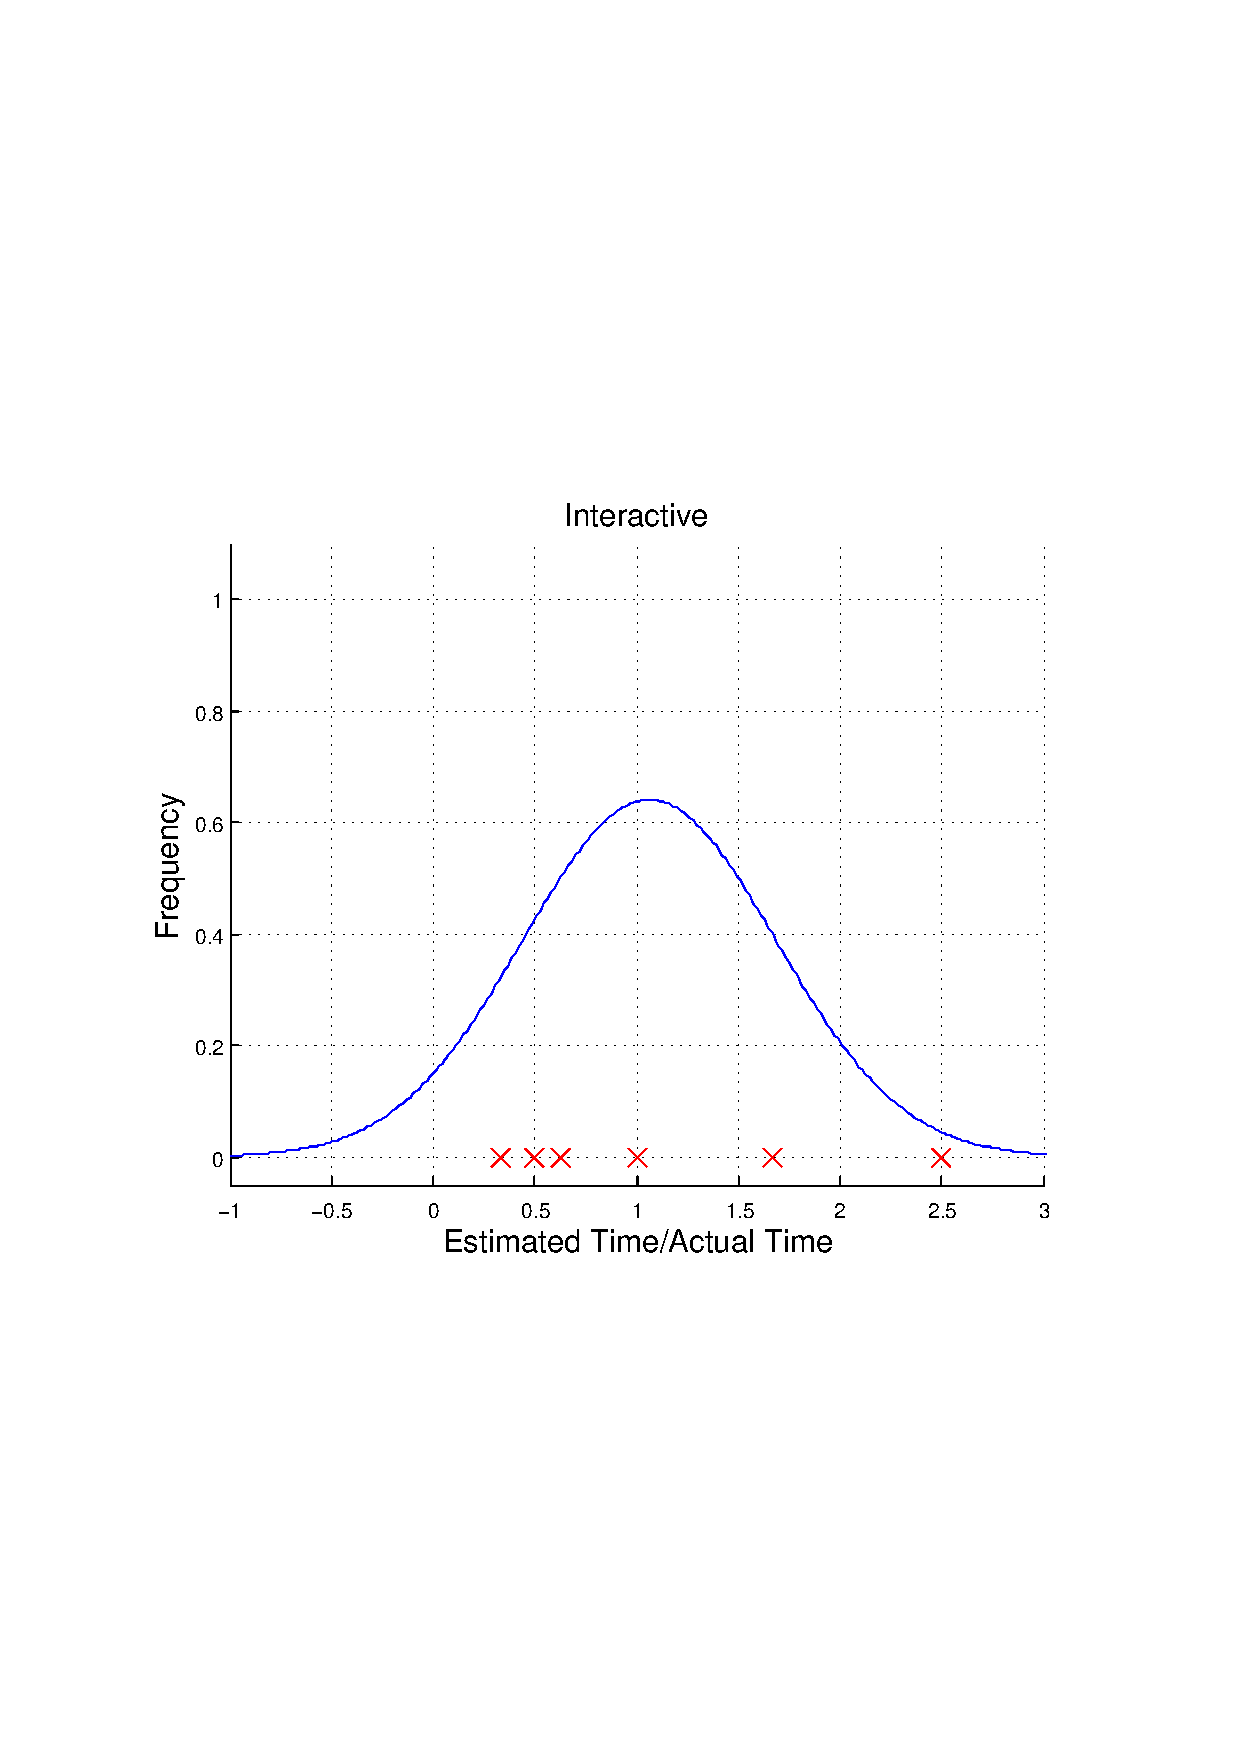
\includegraphics[width=\textwidth]{images/interactive_bell.pdf}
			\caption{Interactive adverts: $\mu=1.0625$, $\sigma=0.6228$}
		\end{subfigure}
		\begin{subfigure}[h]{0.49\textwidth}
			\centering
			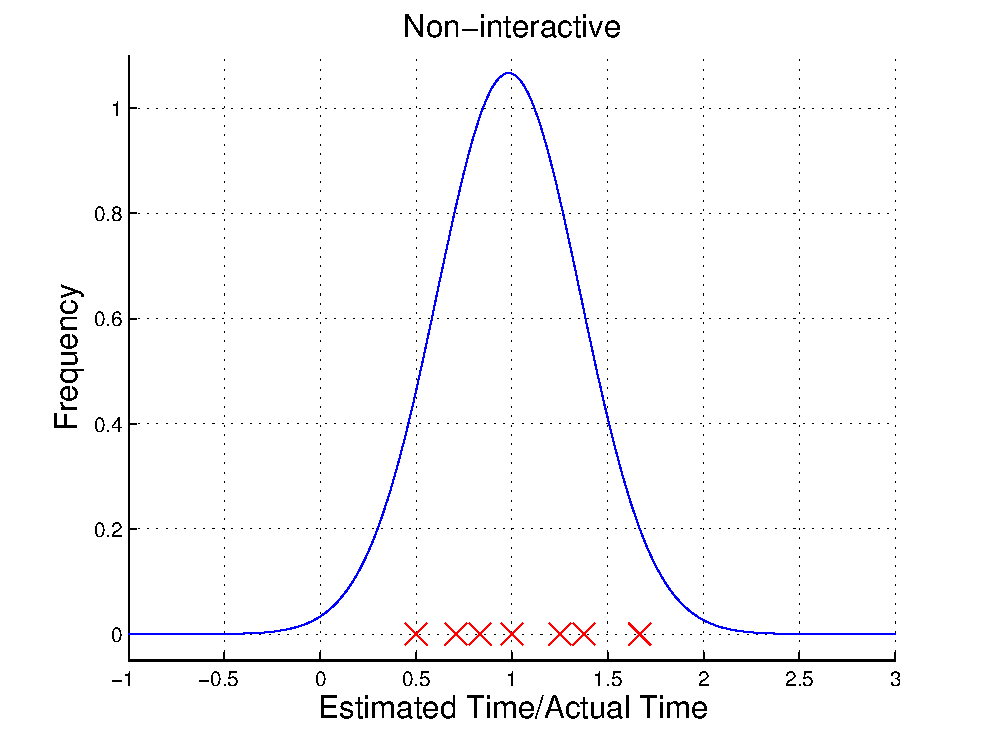
\includegraphics[width=\textwidth]{images/noninteractive_bell.pdf}
			\caption{Non-interactive adverts: $\mu=0.9833$, $\sigma=0.3739$}
		\end{subfigure}
		\caption{Errors in time estimations of users watching interactive and non-interactive advertisements, and extrapolated normal distributions. 10 points recorded in study used.}
		\label{fig:time_perception}
	\end{figure}
	Little difference in time perception between interactive and non-interactive advertisements is shown by Figure~\ref{fig:time_perception}, which is confirmed when a Student's independent two-sample t-test performed on the time estimate data gives 0.17.

	% Recall
	Using information in the participants answers, a table was constructed of adverts that were recalled by participants and whether the participants had seen the advert in the interactive round, the noninteractive round or both rounds. The recall results are given in Figure~\ref{fig:recall}, where it can be seen that participants had a better recall of adverts from the noninteractive round. 
	\begin{figure}[h!]
		\centering
		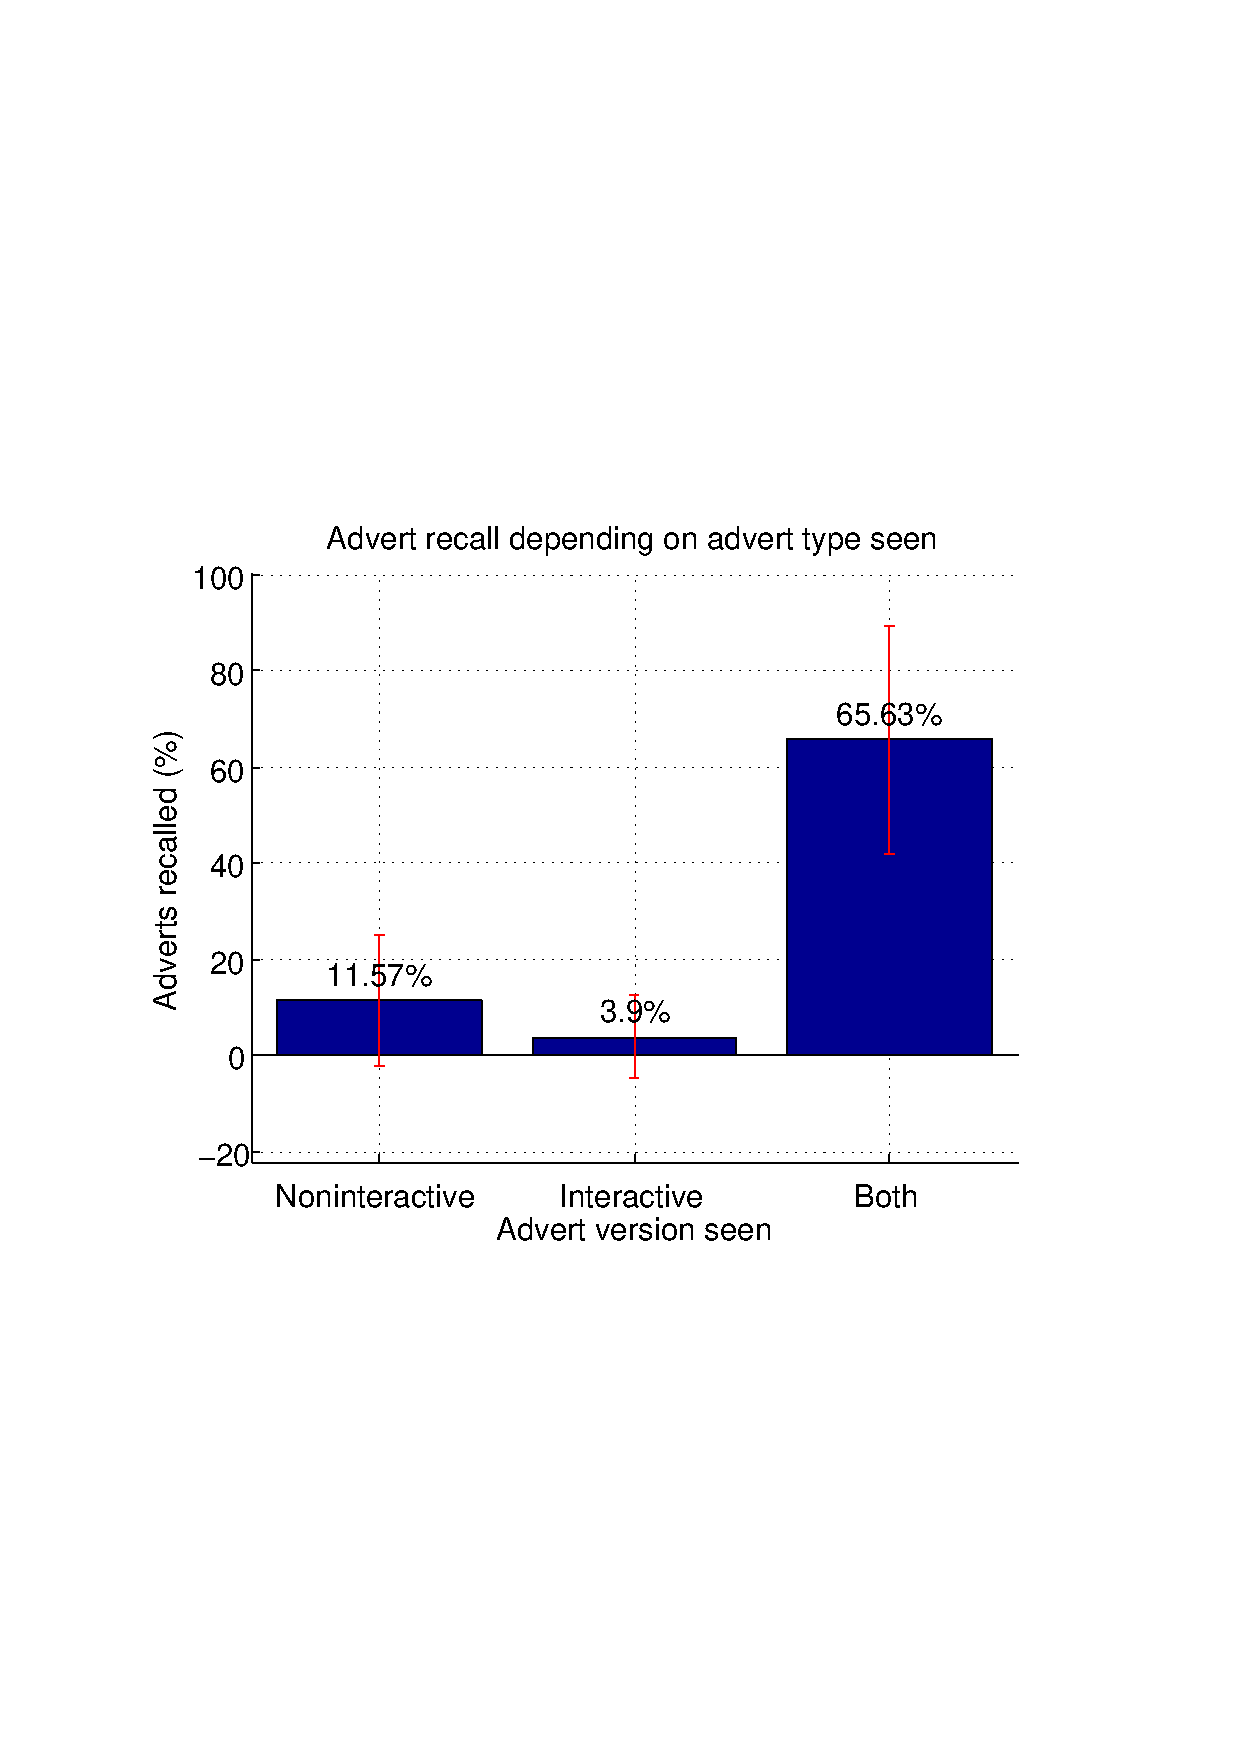
\includegraphics[width=\textwidth]{images/recall.pdf}
		\caption{Average percentage of advertisements recalled depending on the round the advert was seen in (interactive round, noninteractive round or both rounds). The red error bars indicate show the mean recall rate $\pm$one standard deviation.}
		\label{fig:recall}
	\end{figure}

	Along with taking qualitative measurements of time perception and information recall, data were also collected on how participants believed they perceived the interactive and noninteractive adverts differently. This data was collected during the interview stage from participant answers. Questions 3, 4, 5, 6, and 9 were polar (yes/no questions), and the percentage of positive results have been given in Figure~\ref{fig:yesno_results}. The significant results that can be seen from Figure~\ref{fig:yesno_results} are: participants believe that advert relevance leads to heightened attention and likelihood of being watched, and that interactivity in adverts leads to heightened enjoyment. Results which are less significant and with greater variance are: interactive adverts are paid slightly more attention, and are enjoyed marginally less than non-interactive versions.

	\begin{figure}[h!]
		\centering
		\begin{subfigure}[t]{0.49\textwidth}
			\centering
			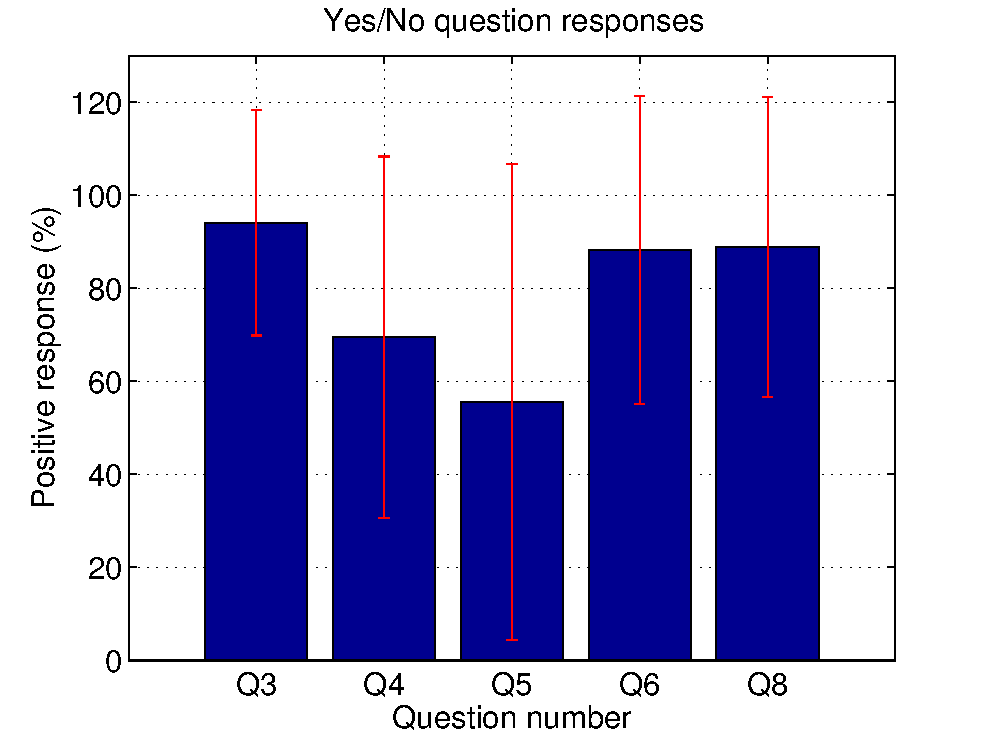
\includegraphics[width=\textwidth]{images/yesno_results.pdf}
			\caption{Positive responses to yes/no questions. \\
				(Q3) More attention paid to relevant ads. \\
				(Q4) More attention paid to interactive ads. \\
				(Q5) Remember more of interactive ads. \\
				(Q6) Enjoyed interactive ads more. \\
				(Q9) More likely to watch relevant ads.
			}
			\label{fig:yesno_results}
		\end{subfigure}
		\begin{subfigure}[t]{0.49\textwidth}
			\centering
			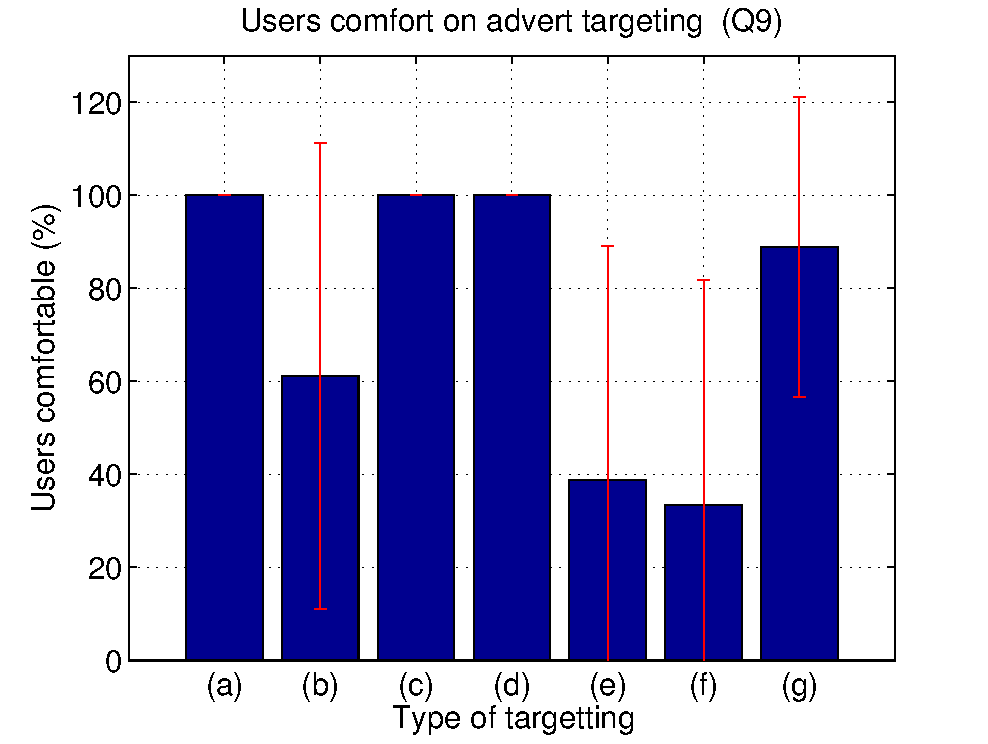
\includegraphics[width=\textwidth]{images/targeting.pdf}
			\caption{Percentages of users who reported to be comfortable with different advert targeting information sources. (a) Anonymous demographics. (b) Current location. (c) Current time. (d) Playlist content. (e) Internet browsing history. (f) Facebook information. (g) User preference information learned by the system.}
		\end{subfigure}
		\caption{Analysis of user answers to a number of questions. The red error bars indicate show the mean values $\pm$one standard deviation.}
		\label{fig:qualitative_results}
	\end{figure}

	The results regarding user time perception and information recall measurements were unexpected. While the hypothesis of heightened user engagement during interactive advertisements is not supported by the evidence gathered during the user study, the significance of the data gathered is not great enough to draw any conclusions, and further study is required.
